\chapter{Files, formats and saving}
\label{ch:files}

MeerK40t speaks more formats than it writes, and the one it writes is not the one
most people expect. This chapter is about getting artwork in, keeping a project
you can come back to, and producing the file your machine actually consumes.

\section{The project file is an SVG}

MeerK40t's own file format is \textbf{SVG} --- the same Scalable Vector Graphics
that Inkscape and Illustrator produce --- extended with extra attributes in a
\file{meerk40t:} namespace. Everything is in there: the elements, the operations
with their settings, the regmarks, and the notes you typed. Saving a project is
therefore saving an SVG, and opening one is opening an SVG.

\begin{description}[leftmargin=1.4em,style=nextline]
  \item[\menu{File>New} (\key{Ctrl+N})] Clears operations, elements and notes.
        Your unsaved work is gone; there is no ``are you sure'' beyond the
        obvious.
  \item[\menu{File>Open Project} (\key{Ctrl+O})] Clears the current project and
        loads a file. Hold \key{Shift} to be asked where the loaded content
        should be placed.
  \item[\menu{File>Import File}] Loads a file \emph{into} the current project
        without clearing anything. This is how you combine artwork from several
        sources into one job. \key{Shift} again offers the placement target.
  \item[\menu{File>Save} (\key{Ctrl+S})] Writes the project to the file it came
        from. If the project has more than one file attached, or the extension is
        not the plain SVG one, Save falls back to Save As.
  \item[\menu{File>Save As} (\key{Ctrl+Shift+S})] Writes to a new file. You get
        three choices: \emph{Scalable Vector Graphics} (the default, with
        MeerK40t's attributes), \emph{SVG-Plain} (no extensions --- a normal SVG
        that other programs will read cleanly, but which loses your operations)
        and \emph{SVG-Compressed} (\file{.svgz}).
\end{description}

\begin{warnbox}[``SVG-Plain'' discards the recipe]
Saving plain is the right move when you want to hand the geometry to another
program. If you open that file again in MeerK40t, you will find the shapes, but
not the operations, the speeds or the notes. Keep the full-fat version as your
working file and export a plain copy when you need to share.
\end{warnbox}

\begin{tipbox}[One project per job, versions when it matters]
The cheapest workflow that scales is: one project file per physical job, named
after the job, saved with a copy for each successful material test
(\file{tag-3mm-ply-v2.svg}). Use \menu{File>Import File} to pull in parts from
your library of reusable drawings rather than rebuilding them.
\end{tipbox}

\section{The Recent list and drag and drop}

\menu{File>Recent} keeps up to twenty files. Each entry loads with the same
behaviour as \menu{File>Open} (clear first), and holding \key{Shift} while
choosing asks for a placement target. Two extra items live in the submenu:
\btn{Clear project on load}, which decides whether a recent file replaces the
current project or merges into it, and \btn{Clear Recent}, which empties the
list.

You can also drop files onto the main window: drag one or several files from your
file manager and MeerK40t loads them all. Anything it does not recognise produces
an error dialog listing the files it rejected --- worth reading rather than
dismissing, because the usual cause is a format that needs an optional dependency.

\section{What can be loaded, and what can be saved}

\begin{center}\small
\begin{tabular}{@{}L{4.0cm}L{3.1cm}L{7.1cm}@{}}
\toprule
\textbf{Filter in the Open dialog} & \textbf{Extensions} & \textbf{Notes} \\
\midrule
\emph{All valid types} & --- & The default; everything below. \\
\emph{Scalable Vector Graphics} & \file{svg}, \file{svgz} & The native format. \\
\emph{SVG (elements only)} & \file{svg}, \file{svgz} & Reads geometry, ignores
MeerK40t's attributes. \\
\emph{Portable Network Graphics}, \emph{Bitmap Graphics}, \emph{EPS Format},
\emph{TIFF Format}, \emph{GIF Format}, \emph{Icon Format}, \emph{JPEG Format},
\emph{Webp Format} & \file{png}, \file{bmp}, \file{eps}, \file{tiff},
\file{gif}, \file{ico}, \file{jpg}/\file{jpeg}, \file{webp} & Raster images.
EPS is read as a bitmap here. \\
\emph{Inkscape supported files} & \file{pdf}, \file{ai}, \file{cdr}, \file{cmx},
\file{wmf}, \file{vsd} and more & Converted through an installed Inkscape
executable. If Inkscape is missing, these formats are not offered. \\
\emph{Drawing Exchange Format} & \file{dxf} & Requires the \cmd{ezdxf} package.
Centring and 3D-polyline reading are preferences. \\
\emph{EZCad2 Files} & \file{ezd} & Galvo job files, including their laser
settings. \\
\emph{LightBurn Files} & \file{lbrn}, \file{lbrn2} & LightBurn projects. \\
\emph{XTool Files} & \file{xcs} & Two variants: with and without the stored laser
settings. \\
\emph{Gcode File} & \file{gcode}, \file{nc}, \file{gc} & Reread a GRBL job. \\
\emph{Engrave Files} & \file{egv} & Lihuiyu/K40 job records. \\
\emph{RDWorks File} & \file{rd} & Ruida job records. \\
\bottomrule
\end{tabular}
\end{center}

\noindent On the way out there is exactly \textbf{one} saver: SVG, in the three
flavours of the Save As dialog. Everything else you might want to produce ---
G-code for a diode machine, an \file{.egv} for a K40, an \file{.rd} for Ruida, an
\file{.lmc} for a galvo --- is a \emph{device job file}, and it is produced by the
job pipeline, not by Save As.

\begin{figure}[htbp]
\centering
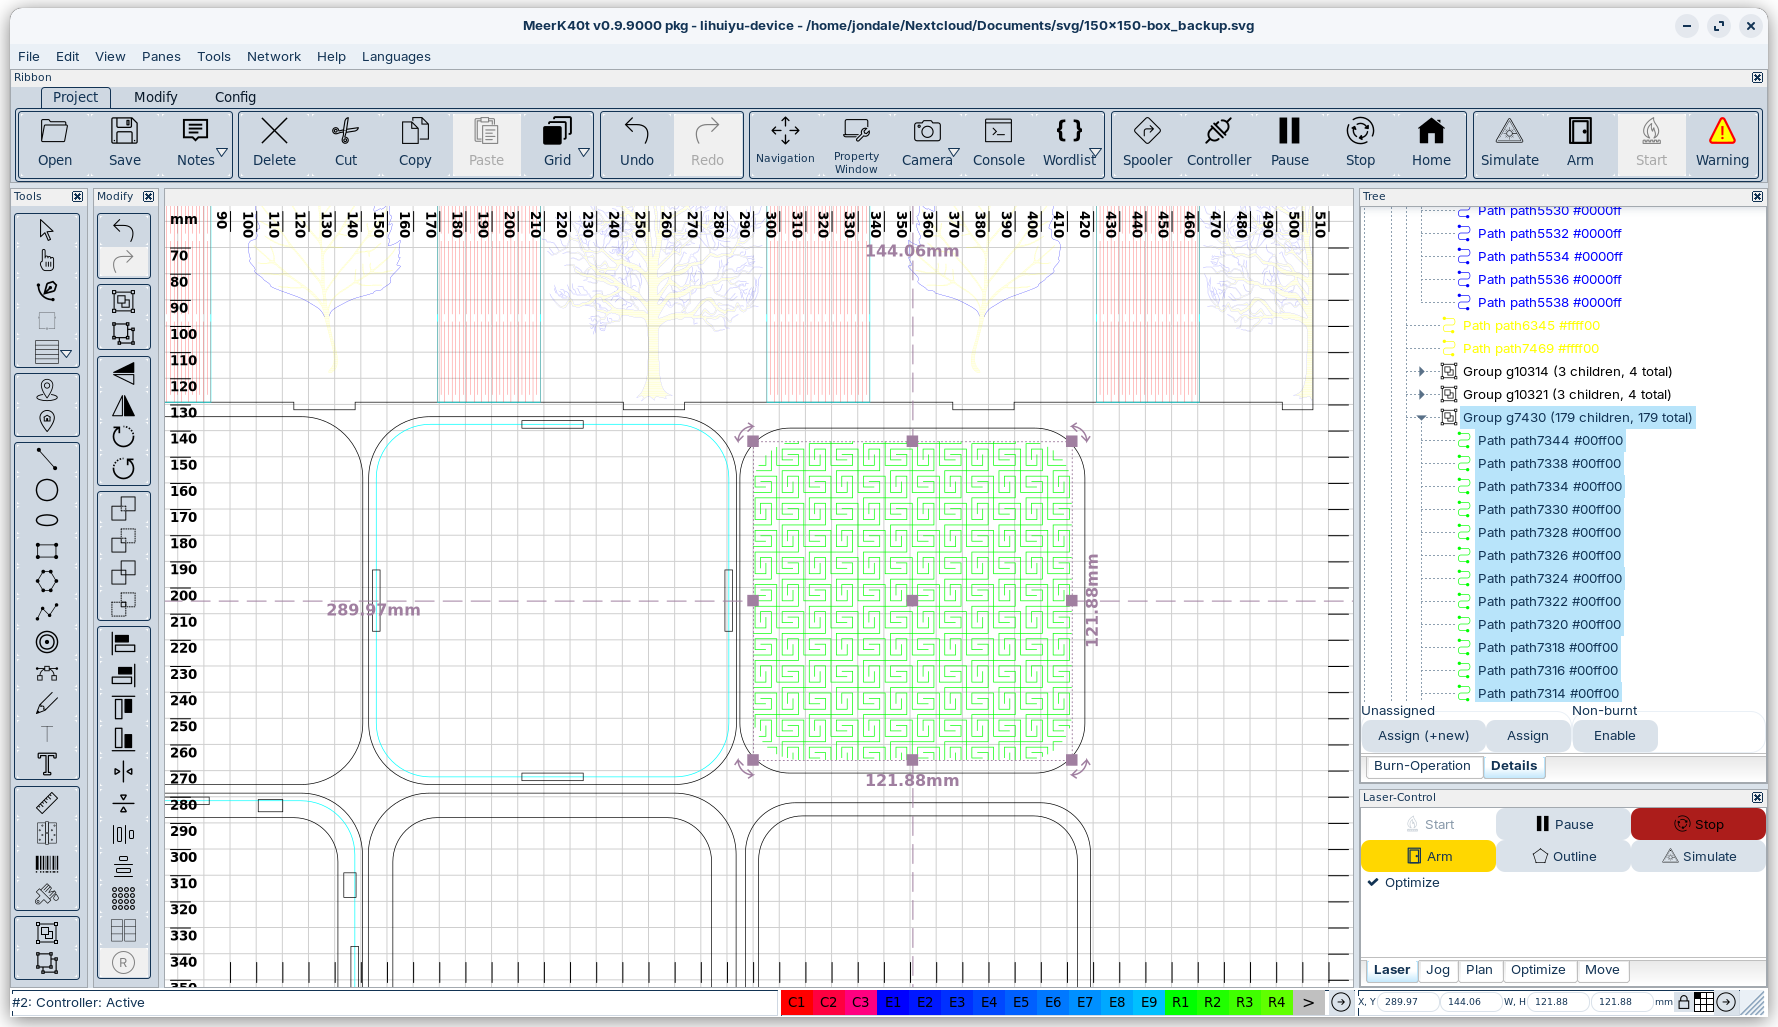
\includegraphics[width=\textwidth]{../screenshots/loaded.png}
\caption{An SVG open in MeerK40t. The tree shows what the file actually
contained: a group with 179 path children, each carrying its stroke colour, and
the scene shows the dimension overlays drawn with the measuring tool. Nothing has
been re-arranged by the import --- this is a faithful reading of the file, which
is exactly why importing good artwork is worth the effort.}
\label{fig:loaded}
\end{figure}

\section{Exporting a machine job file}

\begin{walkthrough}{Produce the file your machine reads}
\begin{enumerate}[label=\arabic*.,leftmargin=1.4em]
  \item Build and optimise the plan as usual (Chapter~\ref{ch:order}).
  \item On the \panel{Laser-Control} pane, open the \tabname{Plan} tab.
  \item Press \btn{Export}. The dialog asks for a file name and offers the
        extension belonging to your active device: \file{.lmc} for a galvo,
        \file{.gcode} for GRBL, \file{.egv} for Lihuiyu, \file{.mos} for Moshi,
        \file{.hpgl} for Newly and \file{.rd} for Ruida.
  \item The export runs in the background; watch the \panel{Console} for
        progress. The plan commands behind the button are
        \cmd{save_job "<path>"} on the current plan.
\end{enumerate}
\end{walkthrough}

\noindent This is how you use MeerK40t as a \emph{design and planning} tool while
running the job from an SD card, a USB stick or the vendor's own software. It is
also the mechanism behind the ESP3D workflow on GRBL machines with Wi-Fi, where
the exported file is uploaded to the controller's SD card and started from its own
panel.

\noindent Lihuiyu users have a bonus pair of commands, \cmd{egv_import <file>} and
\cmd{egv_export <file>}, for reading and writing that format directly from the
console.

\section{Import behaviour and the preferences that change it}

Four preferences change what an import does. They live in
\menu{Edit>Settings>Preferences}, tab \tabname{Input/Output}:

\begin{center}\small
\begin{tabular}{@{}L{5.6cm}L{2.0cm}L{6.6cm}@{}}
\toprule
\textbf{Label} & \textbf{Default} & \textbf{Effect} \\
\midrule
\btn{SVG Viewport is Bed} & on & The SVG's viewport dimensions are used to scale
the rest of the elements. Turn it off if a file arrives at a bizarre size. \\
\btn{Load hidden objects to regmarks} & on & Hidden objects in an SVG are put in
the Regmarks branch rather than loaded as invisible elements. Vector editors use
hidden layers for construction geometry, so this is usually what you want. \\
\btn{Inkscape} & empty & Path to the Inkscape executable, enabling the
Inkscape-supported formats. \\
\btn{Unsupported elements} & \emph{Always load into meerk40t} & What to do with
SVG constructs MeerK40t cannot represent: load them anyway, convert the file with
Inkscape first, or ask at load time. \\
\btn{DXF Center and Fit} & on & Centre a DXF on the bed instead of leaving it at
its own origin. \\
\btn{DXF: Try to read 3D-polylines} & on & Read polylines that carry a Z
coordinate, projected flat. \\
\bottomrule
\end{tabular}
\end{center}

\noindent Image imports have their own preferences --- \emph{Image DPI Scaling},
\emph{Center image on import}, \emph{Scale oversized images} and \emph{Create a
file-node for imported image} --- described in Chapter~\ref{ch:engrave}.

\section{Pasting from other programs}

\key{Shift+Ctrl+V} (\menu{Edit>Paste from system}) is more useful than it looks.
It inspects the clipboard and does the right thing per type:

\begin{itemize}
  \item a bitmap becomes an image element;
  \item text becomes a text element;
  \item a list of files is loaded as if you had dragged them in;
  \item a URL is fetched and placed on the bed.
\end{itemize}

\noindent So ``copy an image from a browser, paste into MeerK40t'' works, and so
does ``copy a path from Inkscape, paste into MeerK40t''.

\section{Autosave, notes and startup commands}

\begin{itemize}
  \item \textbf{Autosave} writes your workspace to \file{\_autosave.svg} in the
        program's working directory every
        \setting{autosave_interval} seconds (default 300, i.e.\ five minutes), if
        \setting{autosave_active} is on. It is a safety net, not a recovery
        system: MeerK40t does not offer to reopen the autosave file at startup,
        so if the program crashes, look for that file yourself and open it
        manually.
  \item \textbf{Notes} attach free text to the project (\panel{Notes} pane,
        \menu{Panes>Tools>Notes}). They are saved inside the project file and,
        with \setting{auto_note} on, the notes pane opens automatically when you
        load a file that has notes. This is the right place for ``cut two of
        these, material is the birch ply from the back shelf''.
  \item \textbf{File startup commands} (\menu{Tools>Auto-Exec}) store console
        commands inside a file and run them when that file is loaded --- handy for
        a project that always needs the same preparation, or for a template you
        hand to other people. The console side is \cmd{file_startup}.
\end{itemize}

\section{The console route}

Everything above has a text equivalent, which is what makes batch work possible:

\begin{lstlisting}[style=konsole]
load /home/me/designs/tag.svg        # load a project or artwork file
save /home/me/designs/tag-v2.svg     # write the project
save /home/me/tag-plain.svg -v plain # write a plain SVG
load_types                           # list everything that can be loaded
save_types                           # list everything that can be saved
plan0 save_job /home/me/tag.egv      # export the device job file
\end{lstlisting}

\begin{tryit}{Assemble one job from three sources}
\begin{enumerate}[label=\arabic*.,leftmargin=1.4em]
  \item \menu{File>New}, then \menu{File>Import File} and load a vector drawing.
  \item \menu{File>Import File} again and load a photograph. Confirm that the
        first drawing is still there --- that is the difference between Open and
        Import.
  \item Paste something from the system clipboard with \key{Shift+Ctrl+V}.
  \item Arrange the three pieces, then \menu{File>Save As} \file{combined.svg}.
  \item \menu{File>Save As} again, this time choosing \emph{SVG-Plain}, and save
        as \file{combined-plain.svg}.
  \item \menu{File>Open Project} the plain file. The geometry is there; the
        operations are gone. That is the value of the extended format --- and the
        reason to keep both.
\end{enumerate}
\end{tryit}
